\capitulo{3}{Conceptos teóricos}

Aunque el proyecto está enfocado a la administración a través de una aplicación web de unos datos que nos facilita el cliente, la base del proyecto se cimienta sobre un algoritmo de optimización capaz de proporcionarnos soluciones acerca de la mejor distribución de plantas energéticas en México. 

La solución proporcionada viene de parte de un algoritmo multiobjetivo llamado NSGA-II\footnote{Nondominated Sorting Genetic Algorithm II}.

\section{NSGA-II}

Implementando esta solución, la meta a la que se quiere llegar es a encontrar un vector de variables x=(x1,x2,…xj) que cumpla con todas las restricciones y condiciones, donde las funciones objetivos resultantes sean optimizadas. \cite{pdf:algoritmo}

Se denomina espacio de solución al conjunto de todas las combinaciones posibles. Es denotado mediante: fn(x)=z=(z1,z2,…zM). 

La diferencia entre problemas de optimizacion monoobjetivo y multiobjetivo, es que en los primeros, una solución se considera mejor que otra si con ella se obtiene una solución objetivo de menor valor si estamos minimizando, o una solución de mayor valor si estamos maximizando.

Sin embargo, en los problemas multiobjetivo, este criterio no es correcto pues entran en juego simultáneamente funciones de minimizar y de maximizar.

Para llegar a una solución, en los problemas multiobjetivo, se introduce un nuevo operador, dominancia. Que define: una solución 
x(1) domina otra solución x(2) si se cumplen las siguientes condiciones. \cite{pdf:nsga-ii}

\begin{itemize}
	\item La solución x(1) no siempre es de menor calidad que x(2) en todos los objetivos.
	\item Al menos en uno de los objetivos, la solución x(1) es estrictamente mejor que x(2).
\end{itemize}

Utilizando estas reglas de manera iterativa sobre un conjunto de soluciones de un probloema de optimización multiobjetivo, se puede llegar a establecer cuales son las alternativas dominantes. Las conocemos como Conjunto No Dominado.
El resto de soluciones pasan a formar parte del Conjunto de Soluciones Dominadas. 

Logrando establecer este conjunto de Soluciones Dominantes en un espacio objetivo, podemos hablar de Frente óptimo de Pareto. (Figura \ref{fig:frentePareto})

\begin{figure}[ht]
	\centering
	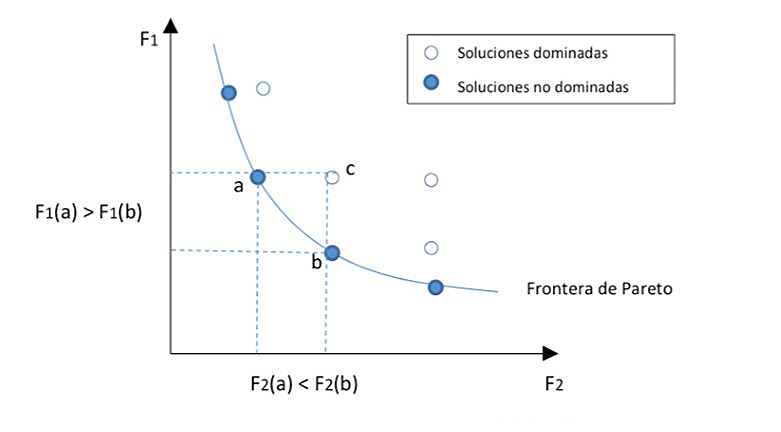
\includegraphics[width=1\textwidth]{/conceptosTeoricos/frentePareto}
	\caption{Frente de pareto en un problema de minimización.\cite{img:frente_pareto}}
	\label{fig:frentePareto}
\end{figure}

\subsection{Pseudocódigo NSGA-II \cite{pdf:nsga-ii}}

\begin{enumerate}
	\item Generar una población P de tamaño N. 
	\item Identificar los frentes de dominancia y evaluar las 
	distancias de apilamiento en cada frente. 
	\item Usando selección (<c)\footnote{Selección por torneo según operador de 
		apilamiento. La selección retorna la solución ganadora i basándose en 
		dos criterios fundamentales.  
		\begin{itemize}
			\item Si tiene mejor rango: ri<rj.
			\item Si tienen el mismo rango pero i tiene mejor distancia de apilamiento: di>d.
		\end{itemize}
	}, cruzamiento y mutación se 
	genera una población descendiente del mismo 
	tamaño de P.  	
	\item Reunir Padres e hijos en un conjunto de tamaño 2N y 
	clasificar los frentes de dominancia. 
	\item Determinar el conjunto descendiente final 
	seleccionando los frentes de mejor rango. Si se 
	supera el límite de población N, eliminar las 
	soluciones con menor distancia de apilamiento en el 
	último frente seleccionado. 
	\item Sí se cumple el criterio de convergencia, Fin del 
	proceso. De lo contrario retornar al paso 3.
\end{enumerate}